%%%%%%%%%%%%%%%%%%%%%%%%%%%%%%%%%%%%%%%%%%%%%%%%%%%%%%%%%%%%%%%%%%%%%
%%
%%%% Gera a apresentação com todas as páginas, links e resumos por seção.
\documentclass[hyphens]{beamer}
%%
%%%% Gera as transparências para os alunos (Somente as páginas de conteúdo).
% \documentclass[trans,hyphens]{beamer}
%%
%%%% Cria um Handout (Folheto / Apostila)
%%\documentclass[handout,hyphens]{beamer}
%%\usepackage{pgfpages}
%%\pgfpagesuselayout{2 on 1}[a4paper,border shrink=5mm]
%%\pgfpagesuselayout{resize to}[a4paper,border shrink=5mm,landscape]
%% 
%%%%%%%%%%%%%%%%%%%%%%%%%%%%%%%%%%%%%%%%%%%%%%%%%%%%%%%%%%%%%%%%%%%%%

%%% Configura o estilo, cores e fonte da apresentação %%%%%%%%%%%%%%%
%%% http://deic.uab.es/~iblanes/beamer_gallery/ %%%

%\usetheme{Marburg} %Marburg %Goettingen
%\usetheme{PaloAlto}
%\usetheme{Madrid}
\usetheme{Darmstadt}
\usecolortheme{rose}  %beaver}  %             % Configura a cor do tema
\usefonttheme{structurebold}                  % Configura a fonte do tema
\setbeamercovered{transparent}                % Configura textos transparentes

%%% Configurações de texto %%%%%%%%%%%%%%%%%%%%%%%%%%%%%%%%%%%%%%%%%%
\usepackage[resetfonts]{cmap}  % Força o arquivo PDF ficar legível para pesquisa e cópia de texto
\usepackage{lmodern}           % Versão melhorada da fonte "Computer Modern"
\usepackage[brazil]{babel}     % Configuração da língua
\usepackage[utf8]{inputenc}    % Configuração dos caracteres de entrada para o TeX
\usepackage[T1]{fontenc}       % Configuração dos caracteres de saída para o PDF

\usepackage{textpos}           % Configurar o posicionamento dos textos
\usepackage{amssymb}           % Lista de símbolos matemáticos

%%-----------------------------------------%%
%% Configuração para formatar código fonte %%
%%-----------------------------------------%%
%\setmonofont{Consolas} %to be used with XeLaTeX or LuaLaTeX
% \usepackage[table]{xcolor}
\definecolor{bluekeywords}{rgb}{0,0,1}
\definecolor{greencomments}{rgb}{0,0.5,0}
\definecolor{redstrings}{rgb}{0.64,0.08,0.08}
\definecolor{xmlcomments}{rgb}{0.5,0.5,0.5}
\definecolor{types}{rgb}{0.17,0.57,0.68}

\usepackage{listings}
\usepackage{listingsutf8}
\lstset{
	% language=C,
	inputencoding=utf8/latin1,
	captionpos=b,
	numbers=left,
	numberstyle=\tiny,
	%frame=lines,
	showspaces=false,
	showtabs=false,
	tabsize=2,
	breaklines=true,
	showstringspaces=false,
	breakatwhitespace=true,
	escapeinside={(*@}{@*)},
	commentstyle=\color{greencomments},
	morekeywords={partial, var, value, get, set},
	keywordstyle=\color{bluekeywords},
	stringstyle=\color{redstrings},
	basicstyle=\ttfamily\scriptsize,
}
%%-----------------------------------------%%


%%% Configurações das imagens %%%%%%%%%%%%%%%%%%%%%%%%%%%%%%%%%%%%%%%
\usepackage{graphicx}          % Posibilitar a inserção de figuras
\graphicspath{{img/}}          % Define o subdiretorio das figuras
\usepackage{epstopdf}          % Permite a inserção de figuras do tipo .eps (Converte EPS para PDF)
\usepackage{tikz}              % Permite incluir imagem na pagina / desenhar figuras

%%% Habilita e configura os hiperlinks %%%%%%%%%%%%%%%%%%%%%%%%%%%%%%
\usepackage{hyperref}


%%% Configura as informações da apresentação %%%%%%%%%%%%%%%%%%%%%%%%%%%%%%%%%%

% Configura as informações da capa
\title[\textit{Devices and Modules}]{Linux - \textit{Devices and Modules}}
\author[Anderson Weller]{Anderson Coelho Weller}
\institute[Unicamp]{Universidade Estadual de Campinas\\Instituto de Computação}
\date{\today}


% Apresenta o número da página atual junto com os botões de navegação
% Obs.: As chaves vazias fazem o número ficar à direita dos botões.
\addtobeamertemplate{navigation symbols}{}{%
    \usebeamerfont{footline}%
	\usebeamercolor[bg]{title}%
    \hspace{1em}%
    \insertframenumber/\inserttotalframenumber
}

% Configura o Logotipo da apresentação
\logo{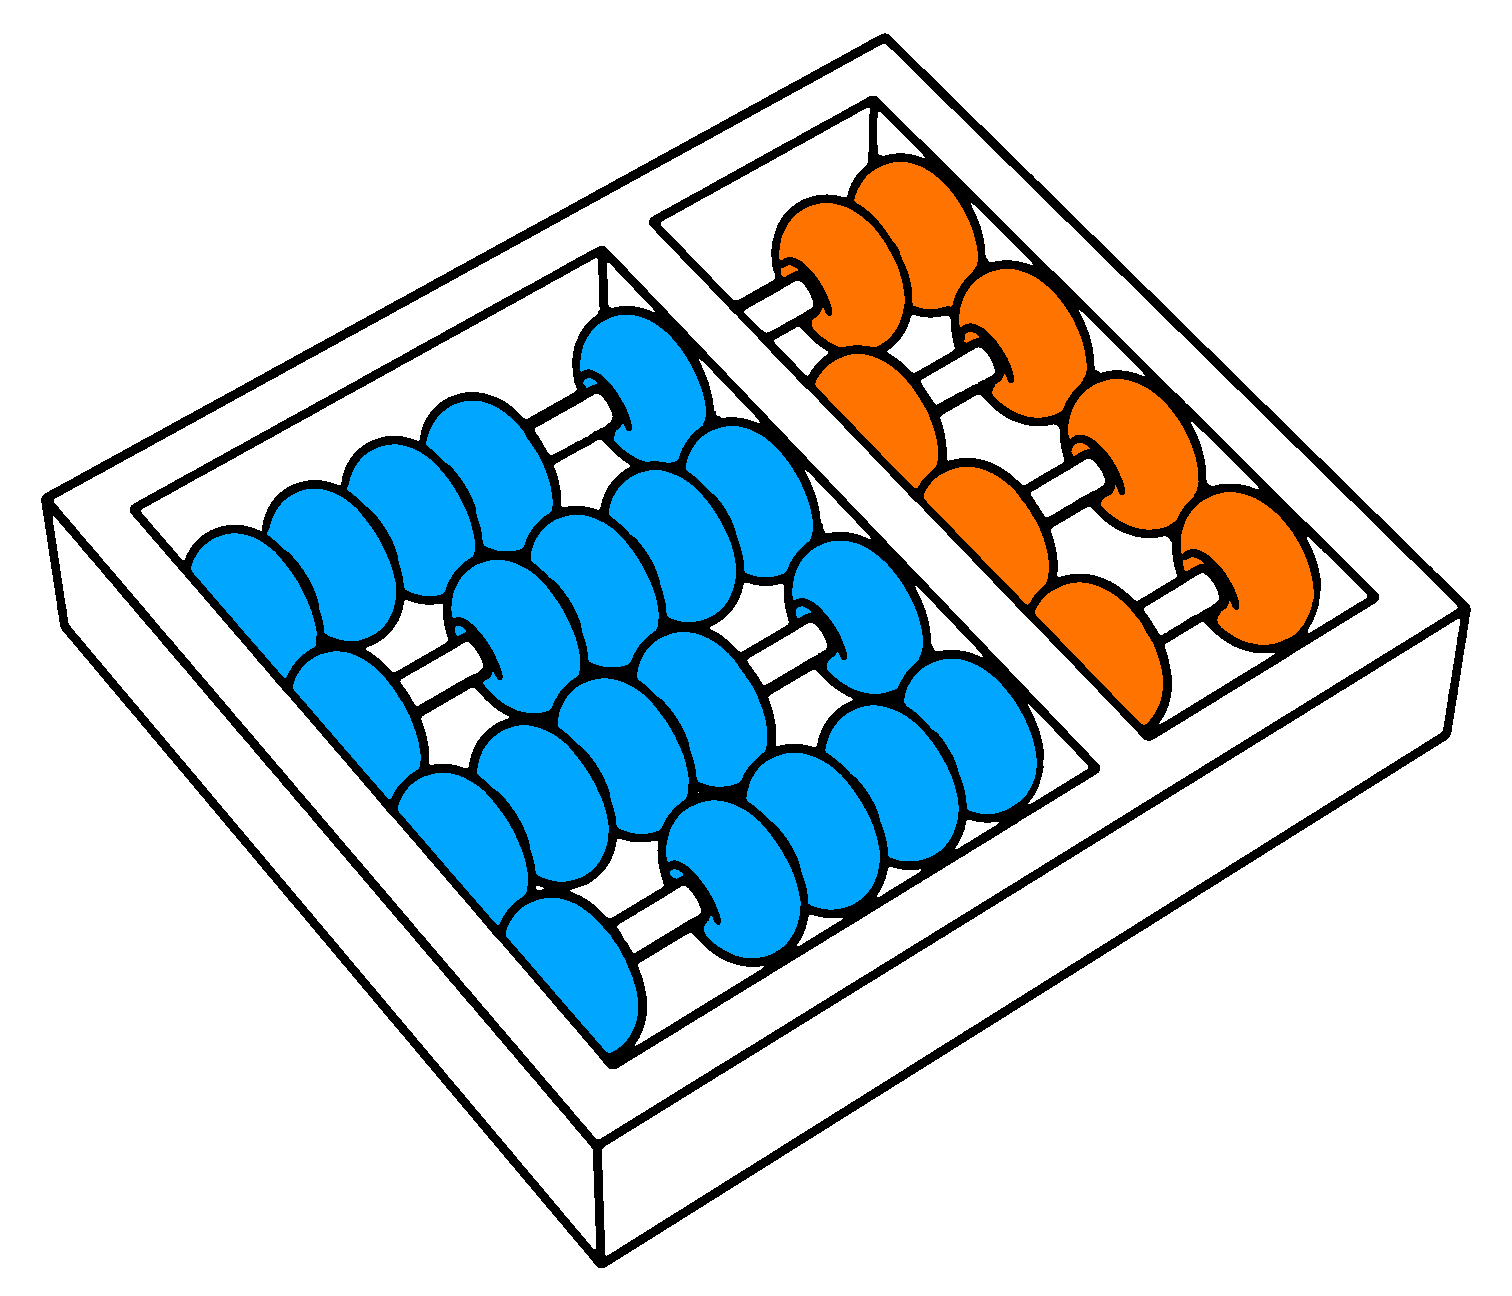
\includegraphics[scale=.014]{logo-ic}}

\begin{document}

%%% Monta a página de título / capa %%%%%%%%%%%%%%%%%%%%%%%%%%%%%%%%%
{
\setbeamertemplate{navigation symbols}{}  %% Oculta a barra de ferramenta na capa
	\begin{frame}

		%%% Monta a capa da apresentação
		\titlepage

		%%% Inclui o logotipo da Unicamp (O logotipo do IC é inserido por "\logo")
		\begin{textblock*}{100mm}(-.07\textwidth,.3cm)
			
\includegraphics[scale=.056]{uec}
		\end{textblock*}
		
	\end{frame}
}


%%% Adiciona o logotipo no título de todas as páginas %%%%%%%%%%%%%%%
%%% Desabilitado pois existe o comando "\logo" (Ver acima)
%\addtobeamertemplate{frametitle}{}{%
%%% Theme: Marburg x Goettingen _________________
%%%\begin{textblock*}{100mm}(.91\textwidth,-.5cm)
%%%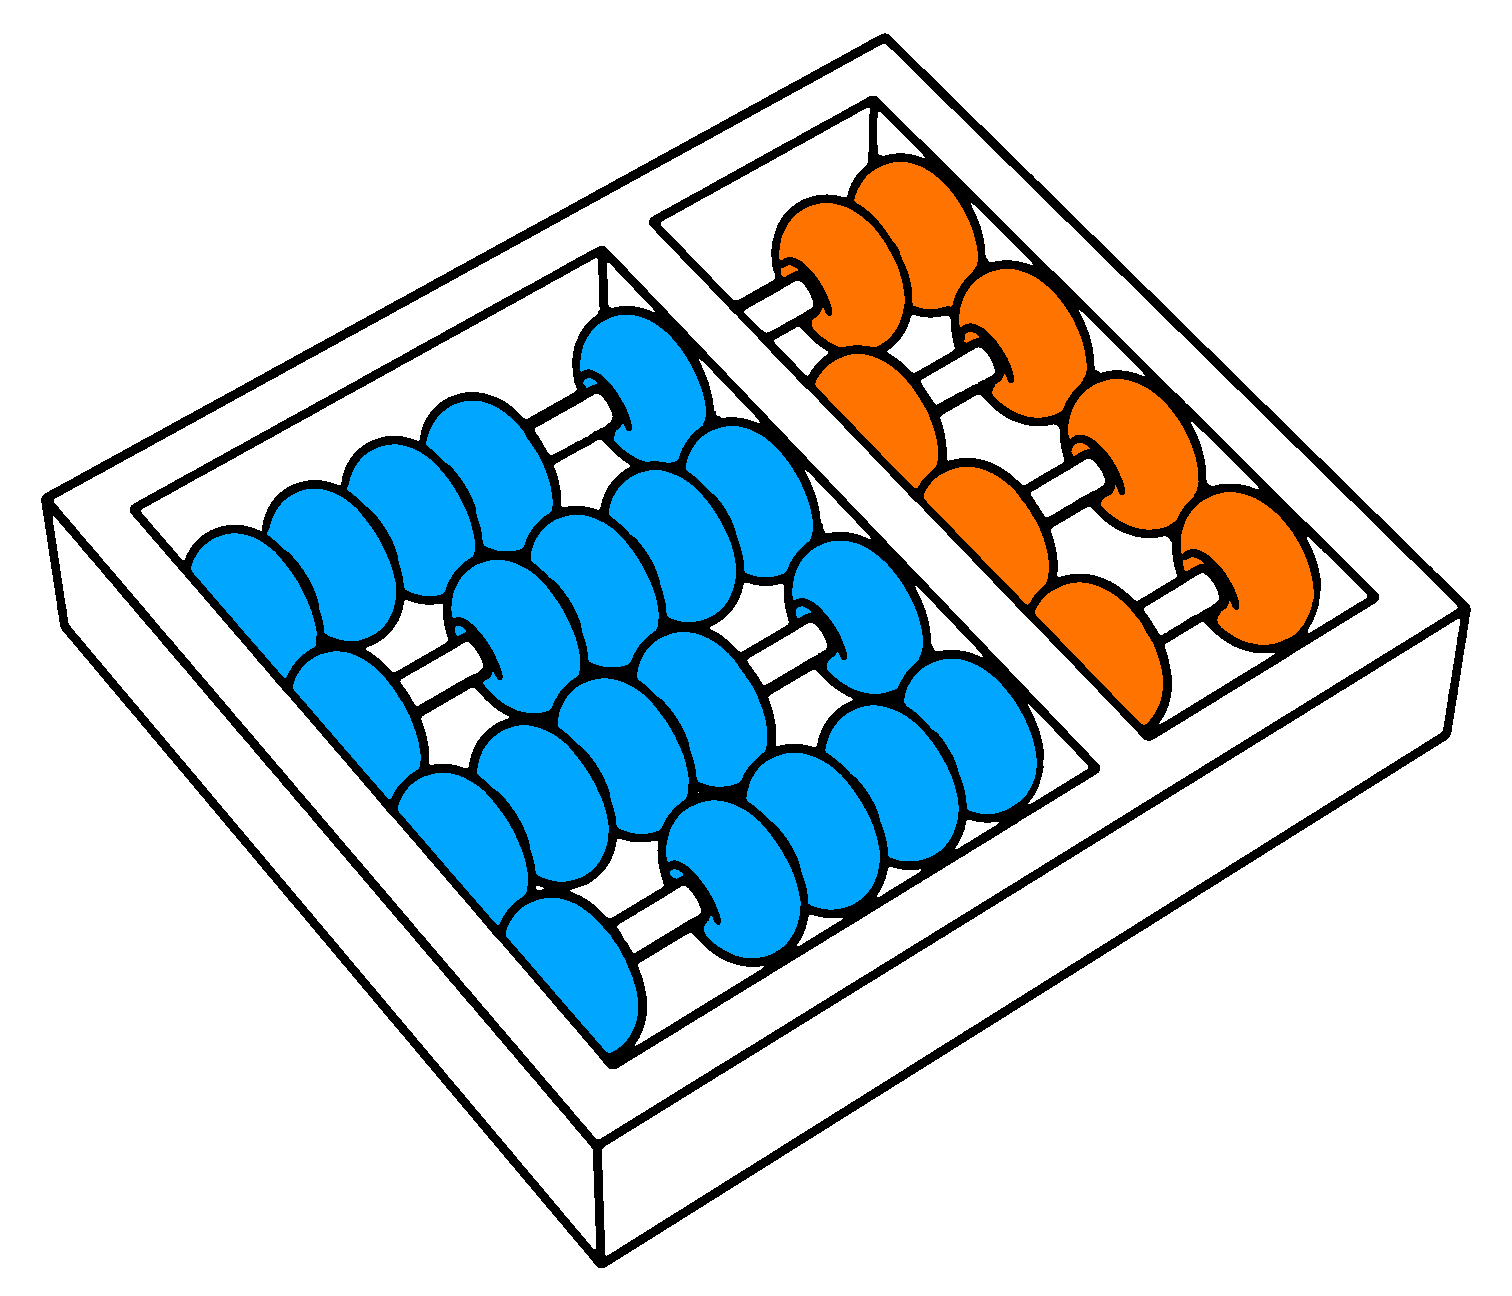
\includegraphics[scale=.022]{logo-ic}
%\end{textblock*}}




%%% Configura uma página de TOC antes de cada seção %%%%%%%%%%%%%%%%%
% %\AtBeginSection[]
% %{
  % \begin{frame}<beamer>
    % \frametitle{Agenda}
	% {
		% %\tiny
		% \tableofcontents %[currentsection] %,currentsubsection]
	% }
  % \end{frame}
% %}

\begin{frame}
	\frametitle{Roteiro}
	\tableofcontents
\end{frame}





%%%%%%%%%%%%%%%%%%%%%%%%%%%%%%%%%%%%%%%%%%%%%%%%%%%%%%%%%%%%%%%%%%%%%
%%% Páginas da apresentação %%%%%%%%%%%%%%%%%%%%%%%%%%%%%%%%%%%%%%%%%
%%%%%%%%%%%%%%%%%%%%%%%%%%%%%%%%%%%%%%%%%%%%%%%%%%%%%%%%%%%%%%%%%%%%%
\section{Devices and Modules} %%%%%%%%%%%%%%%%%%%%%%%%%%%%%%%%%%%%%%%%%%%%%%%%%%%%%%%

\subsection*{Introdução} %%%-----------------------------------------

\begin{frame}
	\frametitle{Classes de Dispositivo}
	\begin{itemize}
		\item<1-> O Linux subdivide os dispositivos em 3 tipos principais:
		\begin{itemize}
			\item<2-> \textit{Character devices} (cdevs)
			\item<2-> \textit{Block devices} (blkdevs)
			\item<2-> \textit{Network devices}
		\end{itemize}
	\end{itemize}
\end{frame}

\begin{frame}
	\frametitle{Classes de Dispositivo}
	\begin{itemize}
		\item<1-> Uma visão geral do \textit{kernel} \cite{LinuxDrivers}
	\end{itemize}
	\begin{columns}[T]
		\begin{column}{.15\textwidth}
		\end{column}
		\begin{column}{.7\textwidth}
			\uncover<1-> {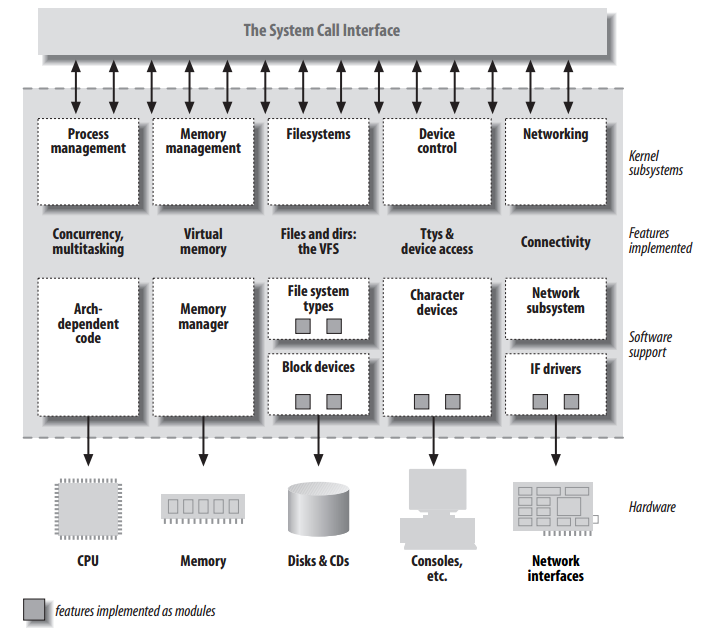
\includegraphics[width=\textwidth]{SplitViewKernel}}
		\end{column}
		\begin{column}{.15\textwidth}
		\end{column}
	\end{columns}
\end{frame}

\begin{frame}
	\frametitle{Classes de Dispositivo}
	\begin{itemize}
		\item<1-> Nem todos os dispositivos são dispositivos físicos.
		\item<2-> Os \textit{pseudo drivers} são dispositivos virtuais que proporcionam acesso à funcionalidades do kernel, tipo:
		\begin{itemize}
			\item<3-> Gerador de números aleatórios do Kernel(/dev/random ou /dev/urandom)
			\item<4-> Dispositivo Null (/dev/null)
			\item<5-> Dispositivo Zero (/dev/zero)
			\item<6-> Dispositivo Full (/dev/full)
			\item<7-> Memória Pricipal (/dev/mem)
		\end{itemize}
	\end{itemize}
\end{frame}

\begin{frame}
	\frametitle{Módulos}
	\begin{itemize}
		\item<1-> Os módulos são imagens binárias (carregáveis no \textit{kernel}) contendo:
		\begin{itemize}
			\item<2-> as sub-rotinas, 
			\item<3-> os dados e 
			\item<4-> os pontos de entrada e saída.
		\end{itemize}
		\item<5-> Que implementam um dos tipos de dispositivos.
	\end{itemize}
\end{frame}


\begin{frame}
	\frametitle{Módulos}
	\begin{itemize}
		\item<1-> O suporte a módulos permite aos sistemas:
		\begin{itemize}
			\item<2-> Manter uma imagem mínima do kernel, e
			\item<3-> Carregar somente os drivers necessários.
		\end{itemize}
	\end{itemize}
\end{frame}

\section{Criar Módulo} %%%%%%%%%%%%%%%%%%%%%%%%%%%%%%%%%%%%%%%%%%%%%%%%%%%%%%%

\subsection*{Instalação} %%%-----------------------------------------

\begin{frame}[fragile]
	\frametitle{Preparação do ambiente}
	
	\begin{itemize}
		\item<1-> Primeiro temos que instalar e preparar os \textit{headers} do \textit{kernel}:
	\end{itemize}

	\lstset{language=bash}

	\begin{block}<1->{}
	\begin{lstlisting}
		sudo -i
		apt-get install module-assistant
		m-a prepare
	\end{lstlisting}
	\end{block}

	\begin{itemize}
		\item<2-> Obs.: O seguinte comando também instala os pacotes que precisamos (equivalente ao ``m-a prepare''):
	\end{itemize}

	\begin{block}<2->{}
	\begin{lstlisting}
		sudo apt-get install build-essential linux-headers-$(uname -r)
	\end{lstlisting}
	\end{block}

\end{frame}


\begin{frame}[fragile, allowframebreaks]
	\frametitle{Arquivo fonte \nocite{}}
	\begin{itemize}
		\item<1-> Crie um diretório e insira o arquivo `hello.c' \cite{KernelDevelopment} \cite{HelloWorld_Mark}, contendo o seguinte código:
	\end{itemize}
	\lstset{frame=lines}
	\lstinputlisting[language=C]{hello.c}
\end{frame}


\begin{frame}[fragile]
	\frametitle{Makefile \nocite{}}
	\begin{itemize}
		\item<1-> Crie o arquivo `Makefile' \cite{HelloWorld_Mark} com as seguintes informações:
	\end{itemize}
	\lstset{frame=lines}
	\lstinputlisting[language={[gnu]Make}]{Makefile.}
\end{frame}


\begin{frame}[fragile]
	\frametitle{Compilar o código}
	
	\begin{itemize}
		\item<1-> Para compilar o código basta executar o `make':
	\end{itemize}

	\begin{block}<1->{}
	\lstset{language=bash}
	\begin{lstlisting}
		make
	\end{lstlisting}
	\end{block}

	\pause

	\begin{itemize}
		\item<1-> Exemplo de retorno do comando `make':
	\end{itemize}

	\lstset{language=TeX, numbers=none}
	\begin{lstlisting}
		make -C /lib/modules/3.2.0-4-686-pae/build M=/home/anderson/modulos modules
		make[1]: Entrando no diretorio `/usr/src/linux-headers-3.2.0-4-686-pae'
		  Building modules, stage 2.
		  MODPOST 1 modules
		make[1]: Saindo do diretorio `/usr/src/linux-headers-3.2.0-4-686-pae'
	\end{lstlisting}

\end{frame}


\begin{frame}[fragile]
	\frametitle{Inserir/Remover Módulo}
	
	\begin{itemize}
		\item<1-> Para inserir o novo módulo no \textit{kernel}:
	\end{itemize}

	\lstset{language=bash}

	\begin{block}<1->{}
	\begin{lstlisting}
		sudo insmod hello.ko
	\end{lstlisting}
	\end{block}

	\begin{itemize}
		\item<2-> Para remover o módulo do \textit{kernel}:
	\end{itemize}

	\begin{block}<2->{}
	\begin{lstlisting}
		sudo rmmod hello
	\end{lstlisting}
	\end{block}

\end{frame}


\begin{frame}
	\frametitle{Inserir/Remover Módulo}
	\begin{itemize}
		\item<1-> Ligando um módulo ao \textit{kernel}:
		\note[item]<1> {gendisk - Representação do disco no Kernel}
		\note[item]<1> {block_device_operations - Conjunto de operações do dispositivo}
	\end{itemize}
	\begin{columns}[T]
		\begin{column}{.05\textwidth}
		\end{column}
		\begin{column}{.8\textwidth}
			\uncover<1-> {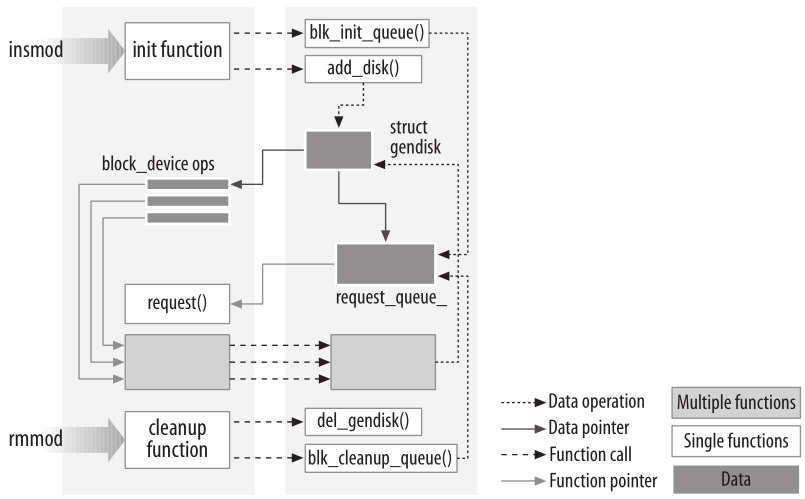
\includegraphics[width=\textwidth]{LinkingModule} \tiny{\cite{LinuxDrivers}}}
		\end{column}
		\begin{column}{.15\textwidth}
		\end{column}
	\end{columns}
\end{frame}


\begin{frame}[fragile]
	\frametitle{Verificar o Log do Linux}
	
	\begin{itemize}
		\item<1-> Verificar as informações do \textit{Log}:
	\end{itemize}

	\lstset{language=bash}
	\begin{block}<1->{}
	\begin{lstlisting}
		tail /var/log/syslog
		# OU
		tail /var/log/messages
	\end{lstlisting}
	\end{block}

	\pause
	
	\begin{itemize}
		\item<1-> Exemplo de conteúdo do \textit{Log}:
	\end{itemize}

	\lstset{language=TeX, numbers=none}
	\begin{lstlisting}
		Nov 11 15:38:35 debian-modulo kernel: Inicio do modulo.
		Nov 11 15:38:40 debian-modulo kernel: Fim do modulo.
	\end{lstlisting}

\end{frame}

\section{Criar CDevs} %%%%%%%%%%%%%%%%%%%%%%%%%%%%%%%%%%%%%%%%%%%%%%%%%%%%%%%

\subsection*{Introdução} %%%-----------------------------------------


\begin{frame}
	\frametitle{\textit{Character devices}}
	\begin{itemize}
		\item<1-> Vamos criar um driver de dispositivo de caractere.
		\item<2-> Esse dispositivo (scull) irá atuar sobre uma área da memória.
		\item<3-> A ideia é demonstrar a interface entre o \textit{kernel} e o dispositivo.
	\end{itemize}
\end{frame}


\begin{frame}
	\frametitle{\textit{Design} do dispositivo}
	\begin{itemize}
		\item<1-> Primeiro, iremos definir as capacidades (o mecanismo) que dispositivo irá disponibilizar para os programas.
		\item<2-> Serão criados os seguintes tipos de dispositivos:
		\begin{itemize}
			\item<3-> \textbf{scull0} a \textbf{scull3}: Área global e persistente da memória, acessível aos programas.
			% \item<4-> \textbf{scullpipe0} a \textbf{scullpipe3}: Dispositivos FIFO, onde um processo lê o que outro grava.
			% \item<5-> \textbf{scullsingle}, \textbf{scullpriv}, \textbf{sculluid} e \textbf{scullwuid}: Parecidos com \textit{scull0}, porém regras para a abertura do dispositivo.
		\end{itemize}
	\end{itemize}
\end{frame}


\begin{frame}
	\frametitle{Números Maiores e Menores}
	\begin{itemize}
		\item<1-> Dispositivos de caractere são acessados pelo nome no sistema de arquivos.
		\item<2-> Eles são arquivos especiais localizados em \textit{/dev}.
		\item<3-> Dispositivos de caractere são identificados pela letra ``c'' (através do comando `\textit{ls -l}')
		\item<4-> Dispositivos de bloco são identificados pela letra ``b''
	\end{itemize}
\end{frame}


\begin{frame}[fragile]
	\frametitle{Números Maiores e Menores}
	\begin{itemize}
		\item<1-> Os dois números que aparecem antes da data de modificação são os números de identificação do dispositivo:
		\begin{itemize}
		
			\note[item]<1> {Esses são os significados tradicionais para esses números.}
			
			\item<1-> \textit{\textbf{Major Number}}: Identifica o driver associado ao dispositivo;
			\item<1-> \textit{\textbf{Minor Number}}: Usado pelo \textit{kernel} para identificar o dispositivo referenciado.
		\end{itemize}
	\end{itemize}
		
	\lstset{language=TeX, numbers=none}
	\begin{block}<1->{}
	\begin{lstlisting}
	    crw-rw-rw- 1 root root  1,   3 Apr 11 2002  null
	    crw------- 1 root root 10,   1 Apr 11 2002  psaux
	    crw------- 1 root root  4,   1 Oct 28 03:04 tty1
	    crw-rw-rw- 1 root tty   4,  64 Apr 11 2002  ttys0
	    crw-rw---- 1 root uucp  4,  65 Apr 11 2002  ttyS1
	    crw--w---- 1 vcsa tty   7,   1 Apr 11 2002  vcs1
	    crw--w---- 1 vcsa tty   7, 129 Apr 11 2002  vcsa1
	    crw-rw-rw- 1 root root  1,   5 Apr 11 2002  zero
	\end{lstlisting}
	\end{block}
	
\end{frame}


\subsection*{Estruturas} %%%-----------------------------------------


\begin{frame}[fragile]
	\frametitle{\textit{Character devices}}
	
	\begin{itemize}
		\item<1-> Para criar um driver de dispositivo de caractere precisamos codificar alguns métodos e ligá-los através das estruturas (ver \cite{LinuxDrivers} e \cite{LDD3_3x}):
		\begin{itemize}
			\item<1-> file\_operations
			\item<1-> seq\_operations
		\end{itemize}
	\end{itemize}

	\lstset{language=C}
	
	\begin{block}<1->{}
		\begin{lstlisting}
			static struct file_operations scull_proc_ops = {
			  .owner   = THIS_MODULE,
			  .open    = scull_proc_open,
			  .read    = seq_read,
			  .llseek  = seq_lseek,
			  .release = seq_release
			};
		\end{lstlisting}
	\end{block}

\end{frame}


\begin{frame}[fragile]
	\frametitle{\textit{Character devices}}
	
	\lstset{language=C}

	\begin{block}<1->{}
		\begin{lstlisting}
			struct file_operations scull_fops = {
			  .owner   = THIS_MODULE,
			  .llseek  = scull_llseek,
			  .read    = scull_read,
			  .write   = scull_write,
			  .unlocked_ioctl = scull_ioctl,
			  .open    = scull_open,
			  .release = scull_release,
			};
		\end{lstlisting}
	\end{block}

	\begin{block}<1->{}
		\begin{lstlisting}
			static struct seq_operations scull_seq_ops = {
			  .start = scull_seq_start,
			  .next  = scull_seq_next,
			  .stop  = scull_seq_stop,
			  .show  = scull_seq_show
			};
		\end{lstlisting}
	\end{block}

\end{frame}


\begin{frame}
	\frametitle{\textit{Scull Device}}
	\begin{itemize}
		\item<1-> Estrutura do dispositivo criado:
	\end{itemize}
	\begin{columns}[T]
		\begin{column}{.15\textwidth}
		\end{column}
		\begin{column}{.7\textwidth}
			\uncover<1-> {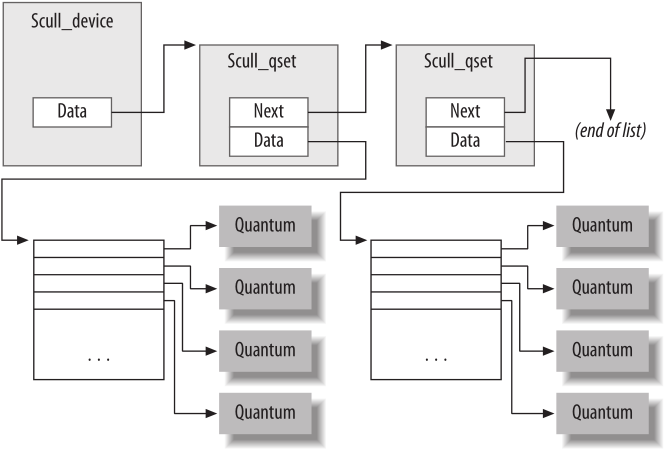
\includegraphics[width=\textwidth]{LayoutScull} \tiny{\cite{LinuxDrivers}}}
		\end{column}
		\begin{column}{.15\textwidth}
		\end{column}
	\end{columns}
\end{frame}


\begin{frame}[fragile]
	\frametitle{\textit{Método de criptografia XOR}}
	
	\begin{itemize}
		\item<1-> Exemplo de criptografia dos caracteres (inserido no método Write) \cite{Codecall_XOR}:
	\end{itemize}
	
	\lstset{language=C}

	\begin{block}<1->{}
		\begin{lstlisting}
			ssize_t scull_read(struct file *filp, char __user *buf, size_t count, loff_t *f_pos) {
			  // (...) Criptografa cada uma das letras da memoria
			  char key[21]   = "12345678901234567890";
			  int  key_count = 0; int  i; int  letra; int  chave;
			  char *buf_ok   = dptr->data[s_pos]+q_pos;
			  for (i=0 ; i<count ; i++)
			  {
			    letra  = buf_ok[i];
			    chave  = key[key_count];
			    buf_ok[i] = letra ^ chave;
			    key_count++;
			    if(key_count == strlen(key))
			      key_count = 0;
			  } // (...)
			}
		\end{lstlisting}
	\end{block}

\end{frame}


%\section{Conclusão} %%%%%%%%%%%%%%%%%%%%%%%%%%%%%%%%%%%%%%%%%%%%%%%%%%%%%%%

\subsection*{Conclusão *** PENDENTE ***} %%%-----------------------------------------

% Conclusão
	% - Lembre ao ouvinte as partes essenciais do que foi apresentado

\begin{frame}
	\frametitle{Conclusão}
	\begin{itemize}
		\item<1-> ...
		\item<2-> ...
		\item<3-> ...
		\item<4-> ...
	\end{itemize}
\end{frame}




%%%%%%%%%%%%%%%%%%%%%%%%%%%%%%%%%%%%%%%%%%%%%%%%%%%%%%%%%%%%%%%%%%%%%
%%% Estrutura proposta pela Ariadne %%%%%%%%%%%%%%%%%%%%%%%%%%%%%%%%%
%%%%%%%%%%%%%%%%%%%%%%%%%%%%%%%%%%%%%%%%%%%%%%%%%%%%%%%%%%%%%%%%%%%%%
% Introdução
	% - Diga sobre o que você vai falar e
	% - Porque esse tema é importante
% Assunto abordado
	% - Apresente o assunto
	% - Ajude o ouvinte a assimilá-lo
% Conclusão
	% - Lembre ao ouvinte as partes essenciais do que foi apresentado

%%%%%%%%%%%%%%%%%%%%%%%%%%%%%%%%%%%%%%%%%%%%%%%%%%%%%%%%%%%%%%%%%%%%%
%%% Estrutura proposta pela Eliane %%%%%%%%%%%%%%%%%%%%%%%%%%%%%%%%%%
%%%%%%%%%%%%%%%%%%%%%%%%%%%%%%%%%%%%%%%%%%%%%%%%%%%%%%%%%%%%%%%%%%%%%
% - Tema
% - Referencia: só se for artigo
% - Tópicos
% - Motivação do trabalho:
     % - qual a importância do trabalho na prática?
     % - qual a relevância teórica do trabalho?
% - Objetivo do trabalho
     % - problema prático a ser resolvido
     % - problema teórico a ser resolvido
% - Técnicas ou trabalhos existentes
% - Solução proposta
     % - o que tem de inovador na solução com relação aos trabalhos existentes?
     % - descrição da solução proposta
           % se possível, com exemplos, no caso de apresentação de artigo
% - Avaliação da solução proposta
    % - como vai mostrar (ou foi demonstrado) que a solução proposta realmente resolve a contento os problemas práticos e teóricos citados no Objetivo: estudo de caso (qual domínio ou aplicação específica)? experimentos (que sujeitos)? avaliação qualitativa ou quantitativa? se quantitativa, quais medidas utilizou (ou vai utilizar)? outros?
% - Pontos em aberto para trabalhos futuros (no caso de apresentação de artigo) ou
   % Metodologia de trabalho
% - Se for um artigo, acrescentar ainda:
    % - pontos fortes: do que voce gostou no artigo?
    % - pontos fracos: do que voce não gostou no artigo?
%%%%%%%%%%%%%%%%%%%%%%%%%%%%%%%%%%%%%%%%%%%%%%%%%%%%%%%%%%%%%%%%%%%%%







%%% Referências %%%%%%%%%%%%%%%%%%%%%%%%%%%%%%%%%%%%%%%%%%%%%%%%%%%%%

\section*{Referências}
\subsection*{Referências}
{
	%%% Ajusta o tamanho das imagens da bibliografia para 65%
	\renewcommand{\pgfuseimage}[1]{\scalebox{.65}{\includegraphics{#1}}}
	
	\begin{frame}[allowframebreaks]
		\frametitle{Referências}
		\bibliographystyle{IEEEtran}
		{
			%\tiny  %%% Diminui o tamanho de letras da bibliografia
			\scriptsize
			%\footnotesize
			%\small
			%\normalsize
			%\large
			%\Large
			%\LARGE
			%\huge
			%\Huge
			\bibliography{90Ref_Linux}
		}
	\end{frame}
}

\subsection*{Agradecimentos}
{ % Monta uma página de encerramento parecida com a de título
	\setbeamertemplate{navigation symbols}{}
	\author{
\includegraphics[scale=.47]{thank-you}}
	\institute{Anderson Coelho Weller}
	\date{}
	\begin{frame}
		\titlepage
		\begin{textblock*}{100mm}(-.07\textwidth,-0.7cm)
			
\includegraphics[scale=.056]{uec}
		\end{textblock*}
	\end{frame}
}

\end{document}
